
\documentclass[../ch1.tex, ../../main.tex]{subfiles}

\usepackage{float}

\begin{document}

    \subsection{Physical and Virtual Addressing}

        The main memory of a computer is organized as an array of $M$ contiguous byte-sized cells. Each byte has a \textit{physical address} (PA). The first byte has an address of $0$, the next byte has an address of $1$, etc. Given this simple organization, it makes sense for a CPU to access memory using physical addresses, an approach known as \textit{physical addressing}.

        \Cref{fig:41} demonstrates an example in the context of a load instruction that reads the $4$-byte word starting at physical address $4$. When the CPU executes the load instruction, it generates an effective physical address and passes it to the main memory over the memory bus. The main memory fetches the $4$-byte word starting at physical address $4$ and returns it to the CPU, which stores it in a register.

        \begin{figure}[H]
            \centering
            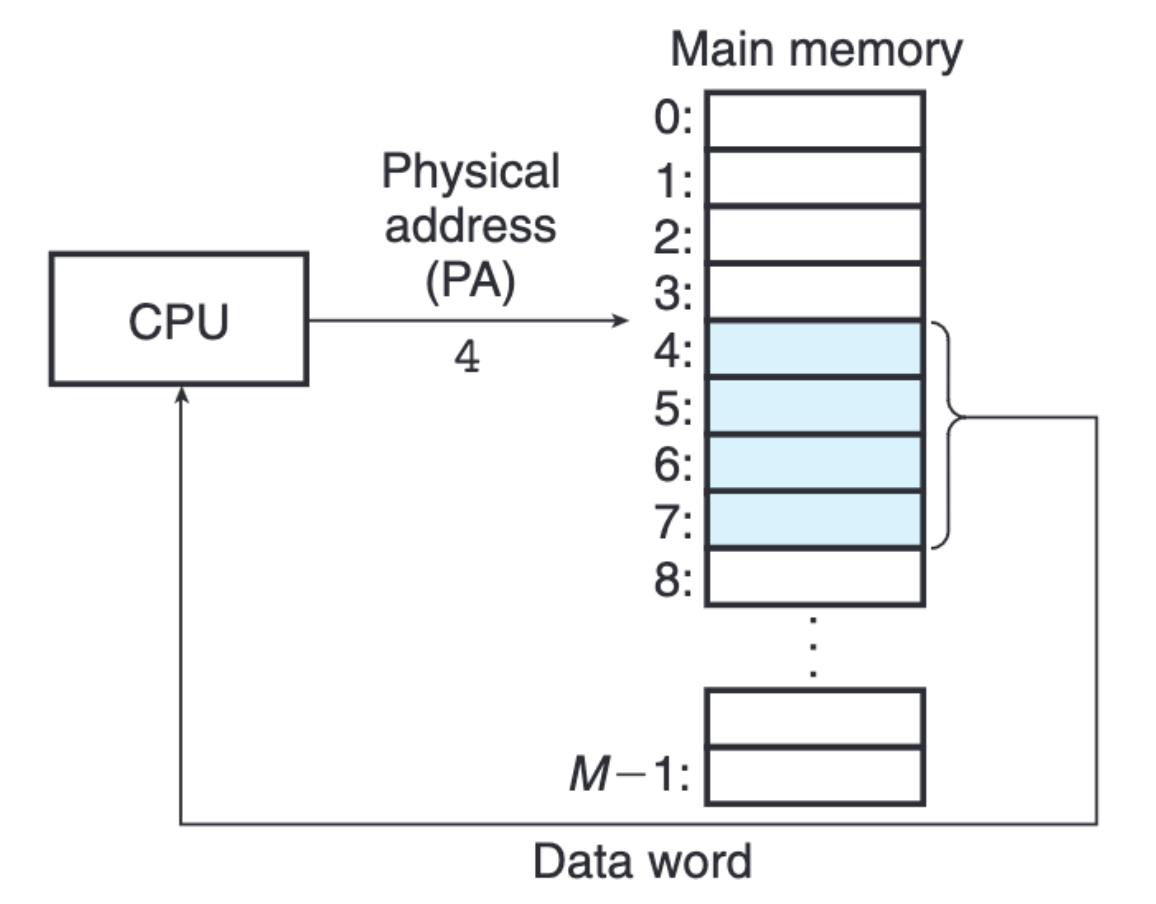
\includegraphics[width=0.75\textwidth]{graphics/Figure 4.1.png}
            \caption{A system that uses physical addressing}
            \label{fig:41}
        \end{figure}

        In contrast, most modern processors use a form of addressing known as \textit{virtual addressing}, shown in \Cref{fig:42}. With virtual addressing, the CPU accesses main memory by generating a \textit{virtual address} (VA), which is converted to the appropriate physical address before being sent to main memory. The task of converting a virtual address to a physical one is known as \textit{address translation}.

        \begin{figure}[H]
            \centering
            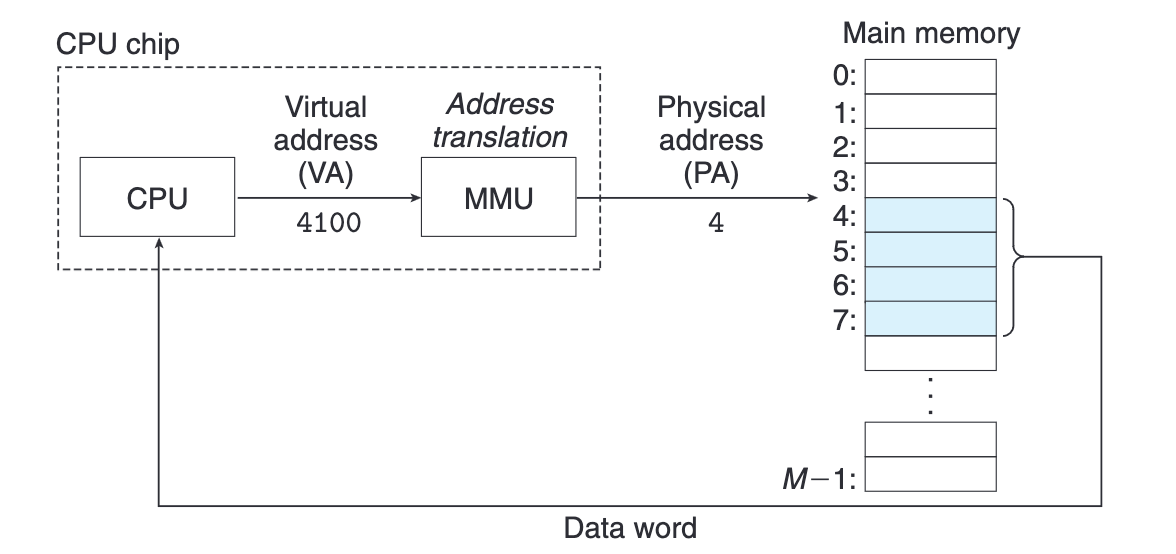
\includegraphics[width=0.75\textwidth]{graphics/Figure 4.2.png}
            \caption{A system that uses virtual addressing}
            \label{fig:42}
        \end{figure}

        Like exception handling, address translation requires close cooperation between the CPU and the operating system. Dedicated hardware on the CPU chip called the \textit{memory management unit} (MMU) translates virtual addresses on the fly, using a lookup table stored in main memory whose contents are managed by the operating system.

\end{document}